% Pacotes e configurações padrão do estilo ``article''\
% -------------------------------------
\documentclass[a4paper,11pt]{article}
% Layout
% ------------------------------------------------------------------------------
%     Gráficos e layout ----------------------------------------------------------------------

\ifx\pdfmatch\undefined
\else
    \usepackage[T1]{fontenc}
    \usepackage[utf8]{inputenc}
\fi
% xetex:
\ifx\XeTeXinterchartoks\undefined
\else
    \usepackage{fontspec}
    \defaultfontfeatures{Ligatures=TeX}
\fi
% luatex:
\ifx\directlua\undefined
\else
    \usepackage{fontspec}
\fi
% End engine-specific settings

%      Fonte --------------------------------------------------------------------------------
%\usepackage{lmodern}
\usepackage{times}
%     Pacotes adicionados -------------------------------------------------------------------
\usepackage{ae}
%     Língua e hifenização ------------------------------------------------------------------
\usepackage[portuguese]{babel}
\usepackage{hyphenat}
%      Outros --------------------------------------------------------------------------------
\usepackage{hyperref} % Permite Links personalisados usando hyperref
\usepackage{fancyhdr}
\usepackage{sectsty}
\usepackage{float}   % Gerencia melhor o posicionamento das figuras e tabelas
%\usepackage{graphicx}
\usepackage[pdftex]{color,graphicx}
\usepackage{hyperref}
\usepackage{enumerate} % Permite alterar Layout do enumerate
%\usepackage{pdflscape}  % Permite alterar a orientação da pagina para Paisagem
%\usepackage{ifthen}  % Permite usar condicionais ifelse
%\usepackage[table]{xcolor} % Permite alterar as cores das células de uma tabela
\usepackage{amsmath,amssymb} % Ambiente para uso de elementos matemáticos
\usepackage{caption}
\usepackage{subcaption} % permite o uso de multiplas figuras com legenda (ambiente subfigure)
\usepackage{minted} % Ambiente minted para colorir código de programas
\usepackage{natbib} % Para referencia bibliográfica
\usepackage{url}    % Referência de links na internet
%\usepackage{listings} % pacote para apresentar código de programação
\usepackage{indentfirst}  % Para indentar o primeiro parágrafo de cada seção
\usepackage{titling}  % Permite Montar uma página de titulo própria

% Layout do documento ------------------------------------------------------------------------
%     Bordas e tamanho da página ------------------------------------------------------------
\usepackage{geometry} 
 \geometry{ % Padrõa ABNT para relatórios
 a4paper,
 left=30mm,
 right=20mm,
 top=30mm,
 bottom=20mm
 }
%     Cabeçalho e Rodapé ---------------------------------------------------------------
\pagestyle{fancy}
  \lhead{}
  \chead{}
  \rhead{}
  \lfoot{}
  \cfoot{}
  \rfoot{\thepage}
%     Númeração ------------------------------------------------------------------------
  \pagenumbering{arabic}
%     Retas do cabeçalho e rodapé ------------------------------------------------------
  \renewcommand{\headrulewidth}{0.5pt}
  \renewcommand{\footrulewidth}{0.5pt}
%     Tamanho da letra de seções e derivadas --------------------------------------------
  \sectionfont{\normalsize}
  \subsectionfont{\small}
%     Hiperlinks ------------------------------------------------------------------------
  \hypersetup{
                  colorlinks,
                  citecolor=black,
                  filecolor=black,
                  linkcolor=black,
                  urlcolor=black
                  }
%     Definições do pdf ----------------------------------------------------------------------
\hypersetup{
    unicode=false,          % non-Latin characters in Acrobat’s bookmarks
    pdftoolbar=true,        % show Acrobat’s toolbar?
    pdfmenubar=true,        % show Acrobat’s menu?
    pdffitwindow=false,     % window fit to page when opened
    pdfstartview={FitH},    % fits the width of the page to the window    
    pdfauthor={Rafael Lima},     % author
    pdfnewwindow=true      % links in new window
}
%     Outros ----------------------------------------------------------------------------
      %\renewcommand{\thesection}{(\alph{section})} % muda o estilo de númeração das sections
      % alterando a formatação dos numeradores de lista de itens
      \renewcommand\theenumi{\arabic{enumi}}
      \renewcommand\labelenumi{(\textit{\theenumi})}
	  \renewcommand\theenumii{\arabic{enumii}}
	  \renewcommand\labelenumii{(\textit{\theenumi.\theenumii})}
      
% ---------------------------------------------------------------------------------------


%\usepackage{circuitikz}

\title{Proposta de projeto - Controle discreto de uma motor DC} % Define o título do Relatório
\author{Rafael Lima}

% Definições Auxiliares ( Macros próprias )
% ------------------------------------------------------------------------------
%\input{relat_aux.tex} % Arquivo com minhas macros
% ----------------------------------~>ø<~---------------------------------------
\begin{document}
% Capa e Índice ----------------------------------------------------------------
%--------------------------------------------------- Capa --------------------------------------------
%\newpage
\begin{figure}[h!]
\centering

\includegraphics[scale=0.9]{img/simb_unb.png}
\label{fig:unb}
\end{figure}

\begin{center}
{\LARGE Universidade de Brasília}\\
Departamento de Engenharia Elétrica\\
Professor: Henrique Cezar Ferreira\\
Disciplina: Controle Digital\\
\end{center}


\vspace{0.18\textheight}

\begin{center}
    \Huge \textbf{\\\thetitle \\}
\end{center}

\vspace*{\fill} % Completa espaço em branco e empurra o resto para o final da página

% Tabela com os nome das pessoas do grupo

\begin{table}[H]
    \begin{tabular}{ll}
        % Nome      & Matrícula
        Rafael Lima & 10/0131093 \\
        Leonardo Cardoso Botelho & 11/0154151 \\
    \end{tabular}
\end{table}

\vspace{0.5cm}

\begin{center}
    \textbf{Brasília\\
    \the\year} % Coloca o Ano atual
\end{center}

\thispagestyle{empty} % Retira o cabeçalho e o rodapé da página

% ------------------------------------------------- Índice -------------------------------------------
\newpage
\tableofcontents
\newpage
% ----------------------------------------------------------------------------------------------------

 % Capa para UnB
% Conteúdo ---------------------------------------------------------------------

\section{Introdução}

A presente proposta de projeto propõe o desenvolvimento de um sistema de controle discreto para uma planta composta por um motor DC (motor de corrente contínua), um sistema de redução e um sensor encoder de maneira a permitir o controle da posição a partir de um sinal de referência.

O motor de corrente contínua é amplamente utilizado em projetos de eletrônica e sua modelagem também está muito bem descrita na literatura de controle em geral. 

Pretende-se aplicar ao fim do desenvolvimento o controlador projetado em uma planta real. O conjunto de peças foi retirada de um equipamento antigo que havia sido descartado. Para implementação do controle, além da planta será utilizado um Arduino UNO e uma módulo com uma ponte H para o controle de potência conforme mostrado na figura \ref{fig:dispositivos}.

\begin{figure}[H]
    \centering
    \begin{subfigure}[b]{0.32\linewidth}
        \centering
        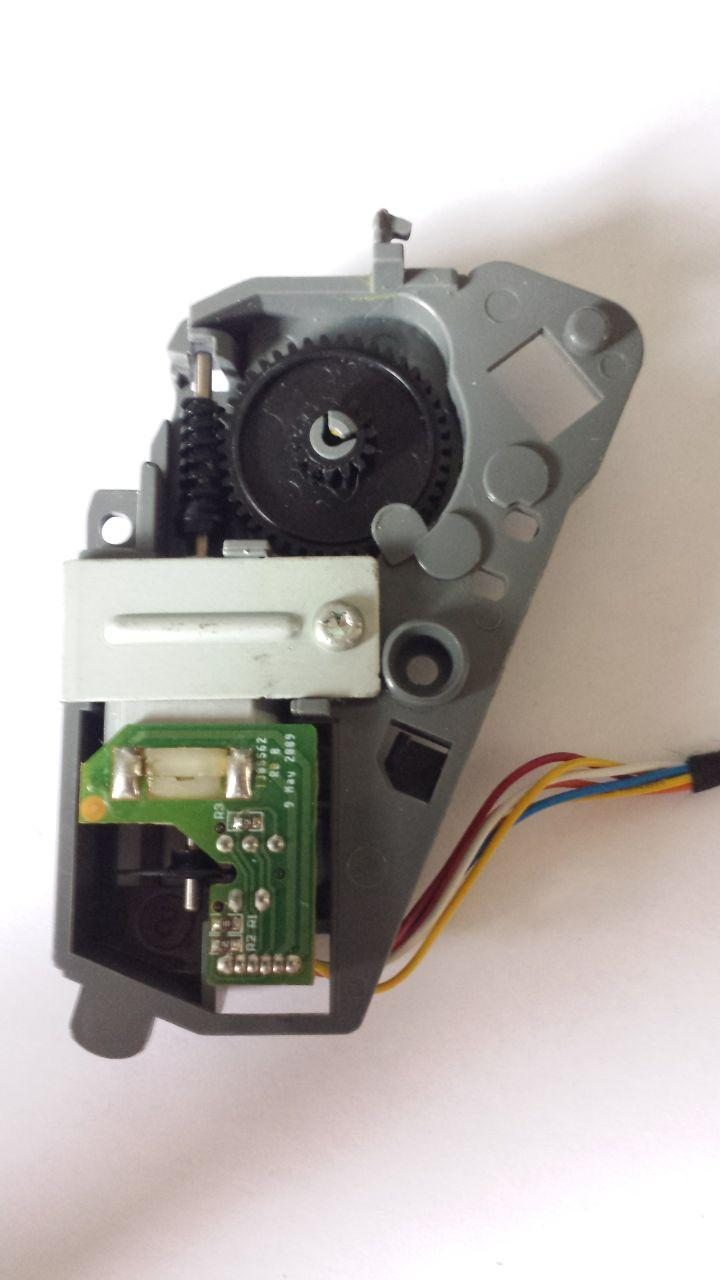
\includegraphics[width=0.8\linewidth]{src/tex/img/servomotor.jpg}
        \caption{Conjunto Motor DC + Encoder}
    \end{subfigure}
    \hfill
    \begin{subfigure}[b]{0.32\linewidth}
        \centering
        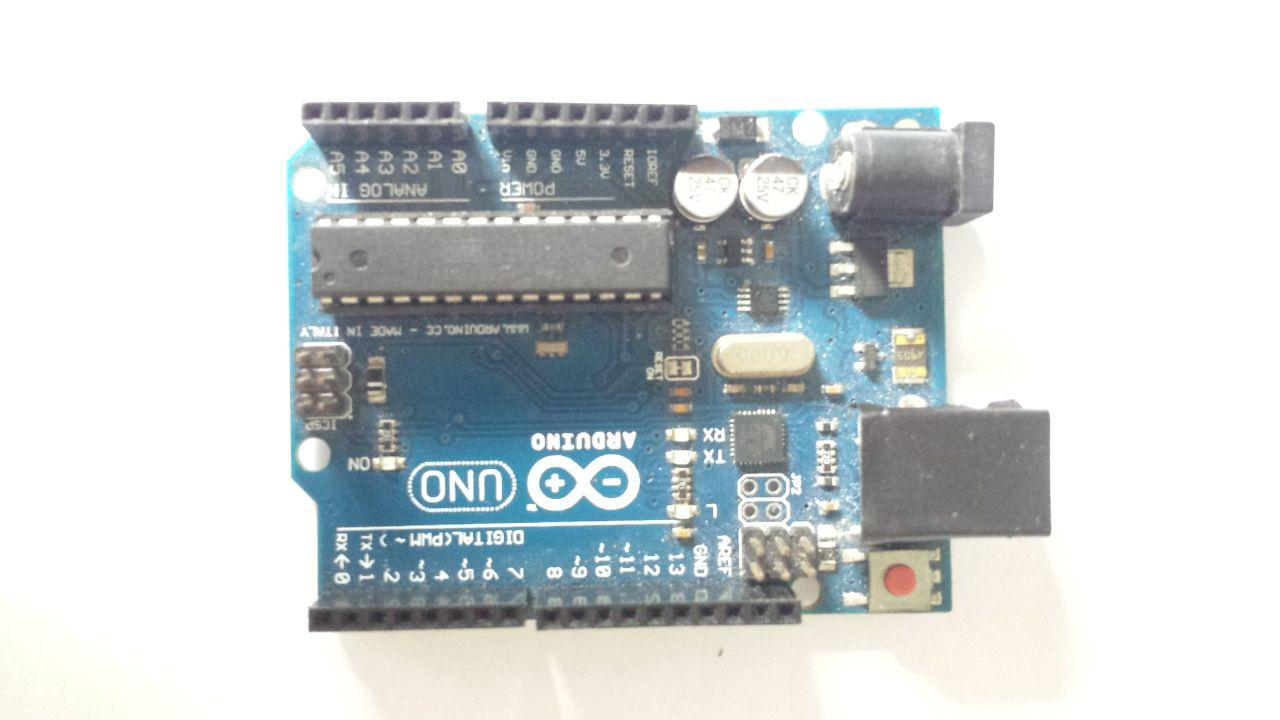
\includegraphics[height=0.9\linewidth, angle=90]{src/tex/img/arduinoUNO.jpg}
        \caption{Arduino UNO}
    \end{subfigure}
    \hfill
    \begin{subfigure}[b]{0.32\linewidth}
        \centering
        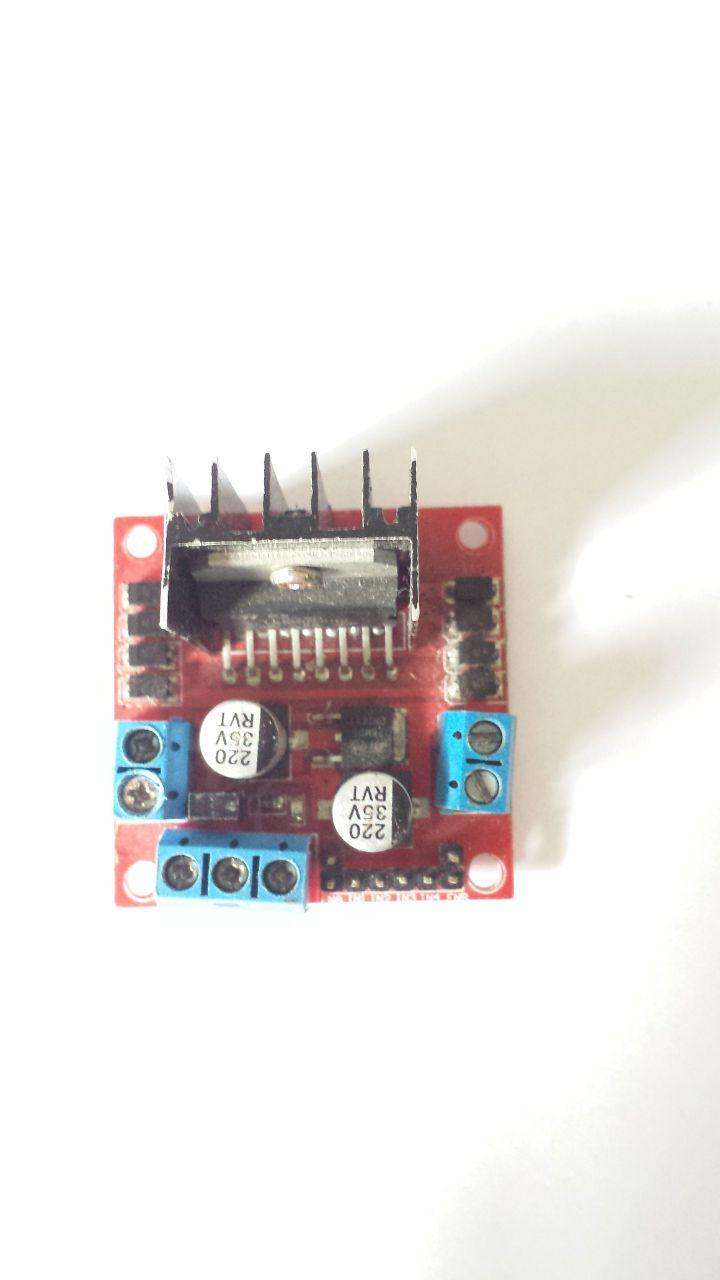
\includegraphics[width=0.9\linewidth]{src/tex/img/ponteH.jpg}
        \caption{Ponte H}
    \end{subfigure}
    \label{fig:dispositivos}
    \caption{Peças para proposta da planta}
\end{figure}

\section{Justificativa}

Sistemas de posicionamento utilizando motores de corrente contínua está presente nos mais variados equipamentos presentes nos dia de hoje. Isso se dá pois eles possuem bom custo benefício, sua implementação e manutenção são facilitadas.

Sua complexidade é razoável para o contexto da disciplina de Controle de Digital pois temos nesse sistema pelo menos dois atrasos nos elementos de atuação e sensoreamento. A caixa de redução por sua vez também insere um aspecto interessante ao processo, visto os efeitos de histerese e zona morta.

Do ponto de vista didático, esse sistema possui bons elementos a serem compreendidos no contexto da disciplina de Controle Digital. Podemos destacar as etapas de modelagem, discretização da planta, alocação de polos no domínio z, projeto em LGR no domínio discreto de um controlador, identificação de sistema e implementação em uma planta real.

Por fim, o controle digital pressupõe um sistema computacional para sua execução, podendo ser operado por um microcontrolador disponível a custo acessível comercialmente. Isso torna esse projeto relevante no contexto das aplicações que utilizam motores de corrente contínua.


\section{Objetivos}

Propõe-se a obter nesse projeto os seguintes objetivos:

 \begin{enumerate}
   \item Obter modelo da planta no domínio da frequência (Motor DC em conjunto com caixa de redução);
   \item Obter modelo do sensor no domínio da frequência;
   \item Obter modelos discreto da Planta e do sensor
   \item Desenvolver modelo em Simulink para o projeto
   \item Obter controlado descrito através de equações de diferenças;
   \item Implementação e Validação do controlador em teste em um sistema real;
 \end{enumerate}

\section{Metodologia de Projeto}

Para o desenvolvimento do projeto foram propostos as etapas relatadas a seguir. Primeiramente será uma revisão bibliográfica e modelagem da planta e avaliação em ambiente de simulação. Num segunda fase será ajustado o modelo encontrado para o planta real.

\begin{itemize}
    \item Estudo Planta Simulada
    \begin{enumerate}
        \item Revisão Bibliográfica para busca do modelo de um servo motor na literatura
        \item Simulação do modelo
        \item Implementação do controle em simulação
    \end{enumerate}
    \item Estudo Planta Real
    \begin{enumerate}
        \item Simulação da planta no Tinkercad
        \item Identificação de Parâmetro da Planta
        \item Simulação da planta a partir do modelo identificado
        \item Implementação do controle em simulação
        \item Implementação do controle na planta
    \end{enumerate}
\end{itemize}

% ------------------------------------------------------------------------------
\newpage
% Referências
\addcontentsline{toc}{section}{Referências} % Adiciona linha no indice
\bibliographystyle{abbrv} % Define Estilo e gera bibliografia
\bibliography{references} % Adiciona Arquivo com Referências

% Acrescentadas no arquivo references.bib
% para usa-las no texto basta usar \citep{}
% para citar sem usar no texto basta usar \nocite{}
%\nocite{sympy}
%\nocite{pythontex}
%\nocite{matlabcontrol}
%\nocite{matlabsymbolic}
\nocite{ogata2010modern}

% ------------------------------------------------------------------------------
%\newpage
%\section*{Anexos}
%\addcontentsline{toc}{section}{Anexos} % Adiciona linha no indice
%\subsection*{Python}

%Para os cálculos e demonstrações foi utilizado o pacote \textit{Python}\TeX\ \cite{pythontex} para o \LaTeX\ em conjunto da bibliteca \textit{sympy}\cite{sympy}. Segue o script completo em python:

%\inputminted[xleftmargin=15pt,linenos,frame=single,framesep=5pt,breaklines=true]{python}{../python/exsim6.py}

%\newpage
%\subsection*{Matlab}

%\subsubsection*{Parte 1}
%Para o desenho dos gráficos e simulações foi utilizado o \textit{Matlab} em conjunto das toolbox \textit{Control System}\cite{matlabcontrol} e \textit{Symbolic Math}\cite{matlabsymbolic}. Segue o código referente usado

%\inputminted[xleftmargin=15pt,linenos,frame=single,framesep=5pt,breaklines=true]{matlab}{../matlab/project.m}

%\newpage
%\subsection*{Arduino}
%Para implementação do controlador foi usado o seguinte código

%\inputminted[xleftmargin=15pt,linenos,frame=single,framesep=5pt,breaklines=true]{c++}{../arduino/pid_control/pid_control.ino}

%\inputminted[xleftmargin=15pt,linenos,frame=single,framesep=5pt,breaklines=true]{c++}{../arduino/pid_control/pid_control.ino}

% ------------------------------------------------------------------------------
\end{document}
